\begin{figure}[tb]
	\begin{center}
		\vspace{-.35in}
		\hspace*{-0.5cm}
		\begin{tabular}{   c | c  c   }
			%\hline
			&\vspace{-.1in}&\\
			& \small{\textsf{Single Frame}} &\small{\textsf{ Unwrapped }}       \\ 
			&\vspace{-.1in}&\\
			& \small{\textsf{with Overlaid Circle}} &\small{\textsf{Space $\times$ Time Image }}       \\ \hline
			&\vspace{-.1in}&\\
			\multirow{1}{*}[0.5in]{ \rotatebox[origin=t]{90}{\small{\textsf{ Truth }} }}
				&
				{{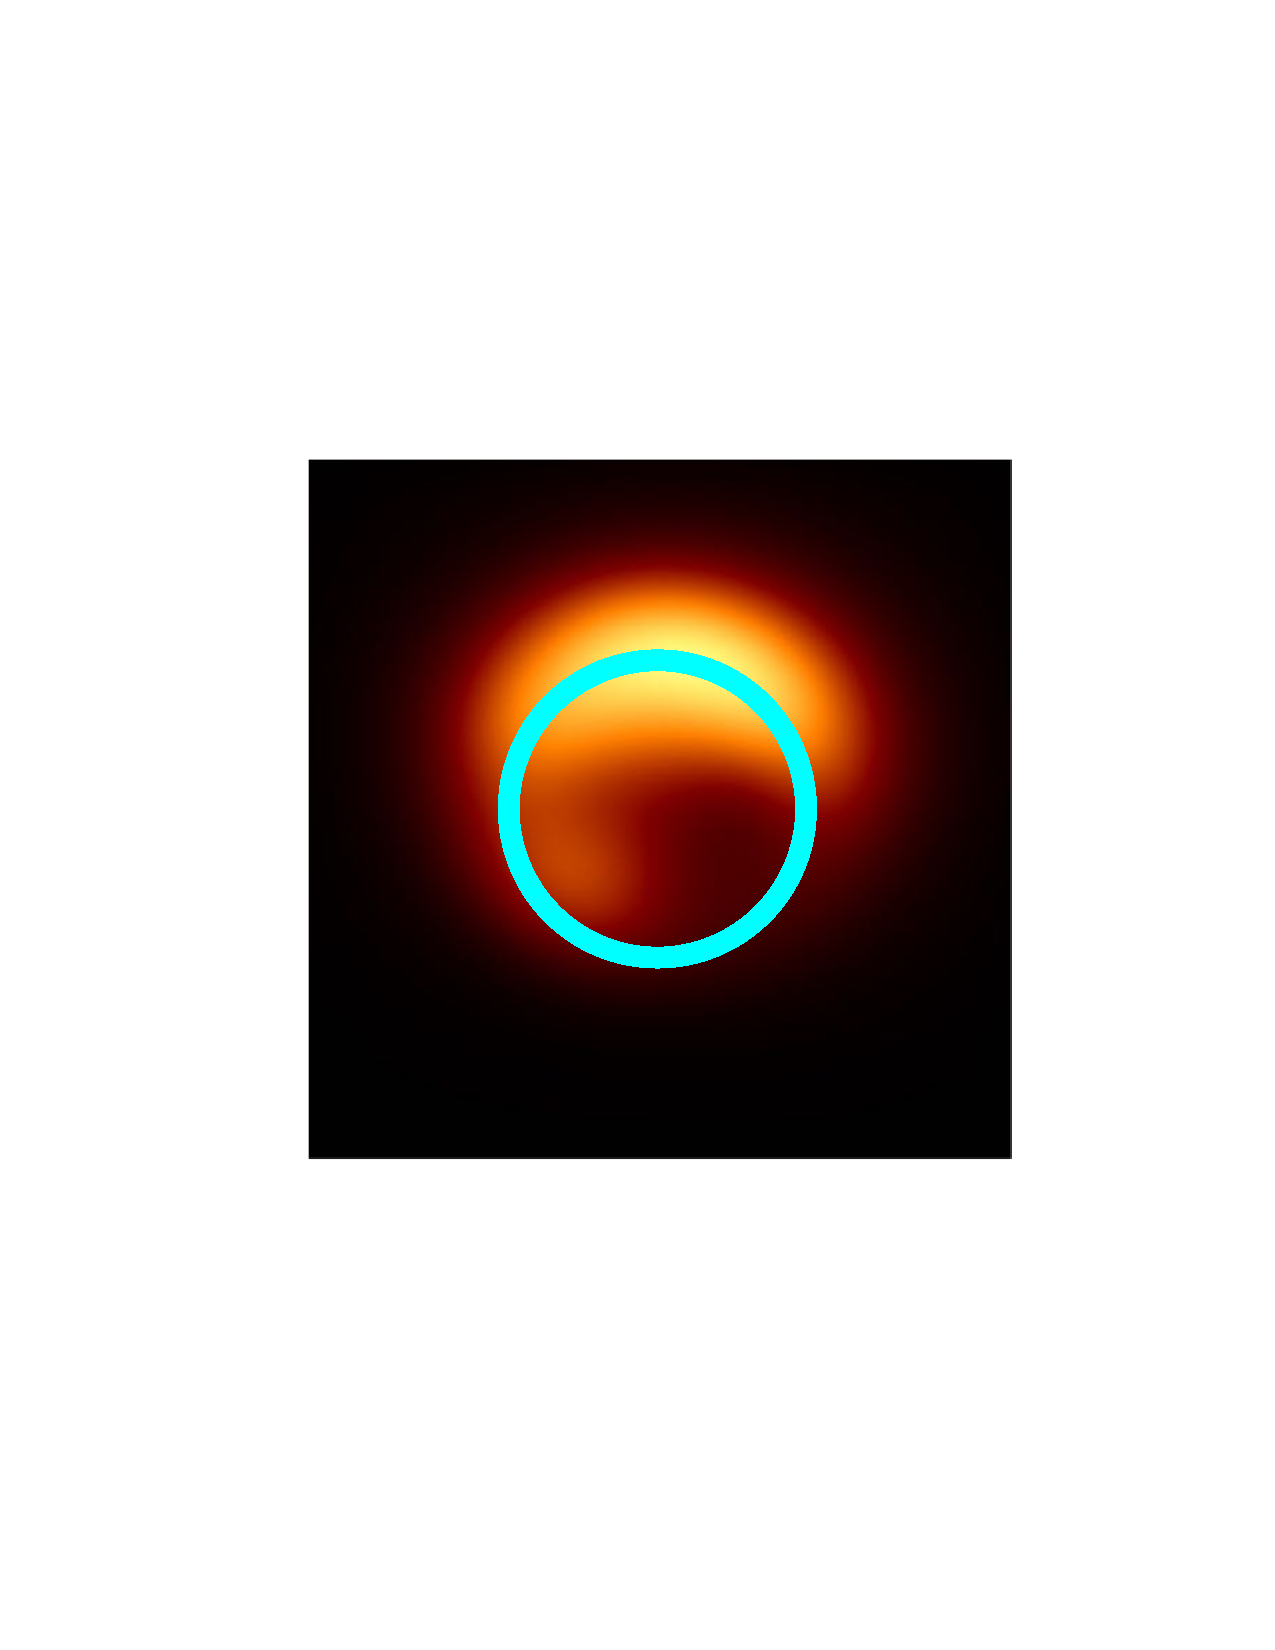
\includegraphics[height=.2\linewidth]{figures/hotspotcircleinterp/groundtruth.pdf}} } &
				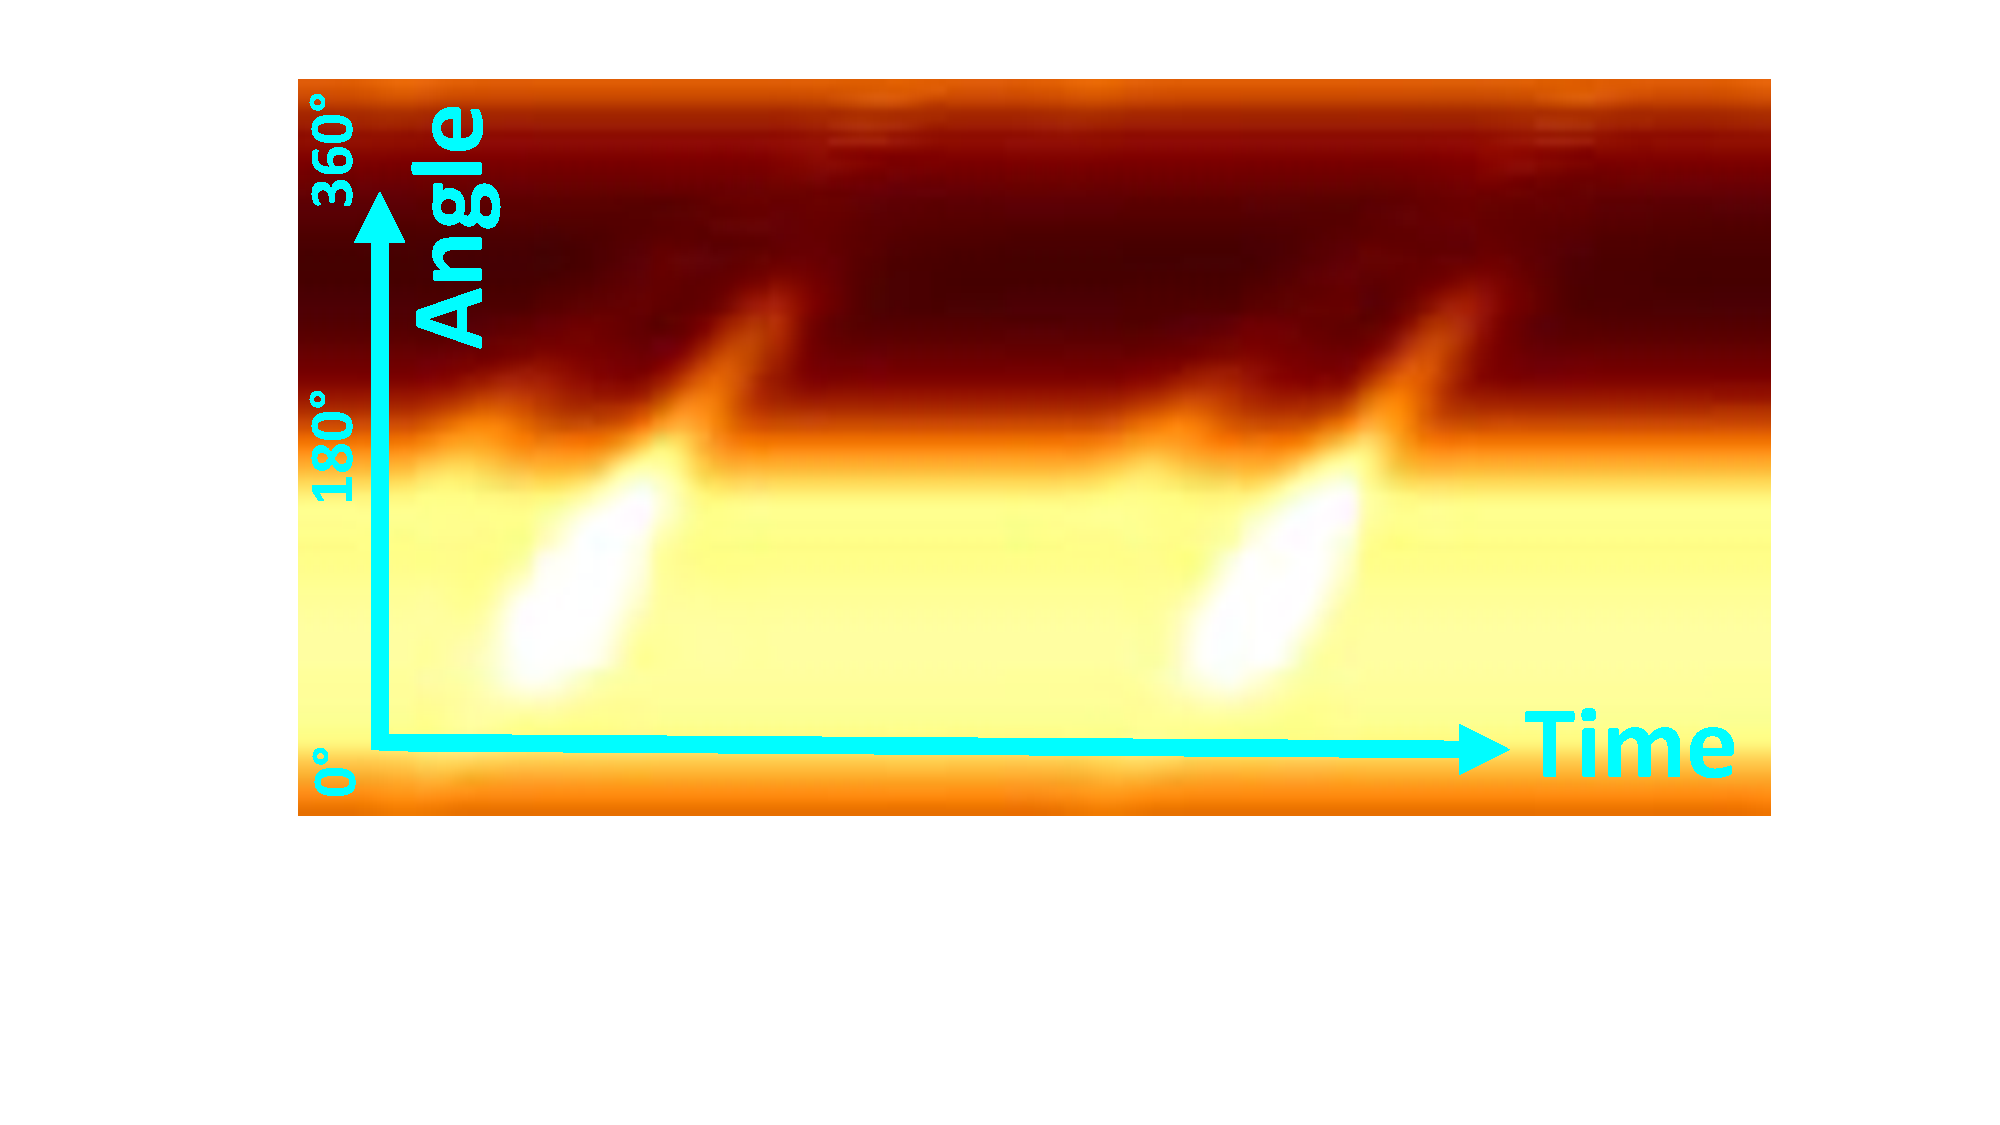
\includegraphics[height=.2\linewidth]{figures/hotspotcircleinterp/labels.pdf} 
				\\
				&\vspace{-.1in}&\\
				\multirow{1}{*}[0.65in]{ \rotatebox[origin=t]{90}{  \specialcell{ \small{\textsf{Blurred Truth}} \\  \tiny{\textsf{ $\frac{3}{4}$ Nominal Beam}}}  }}
			&
			{{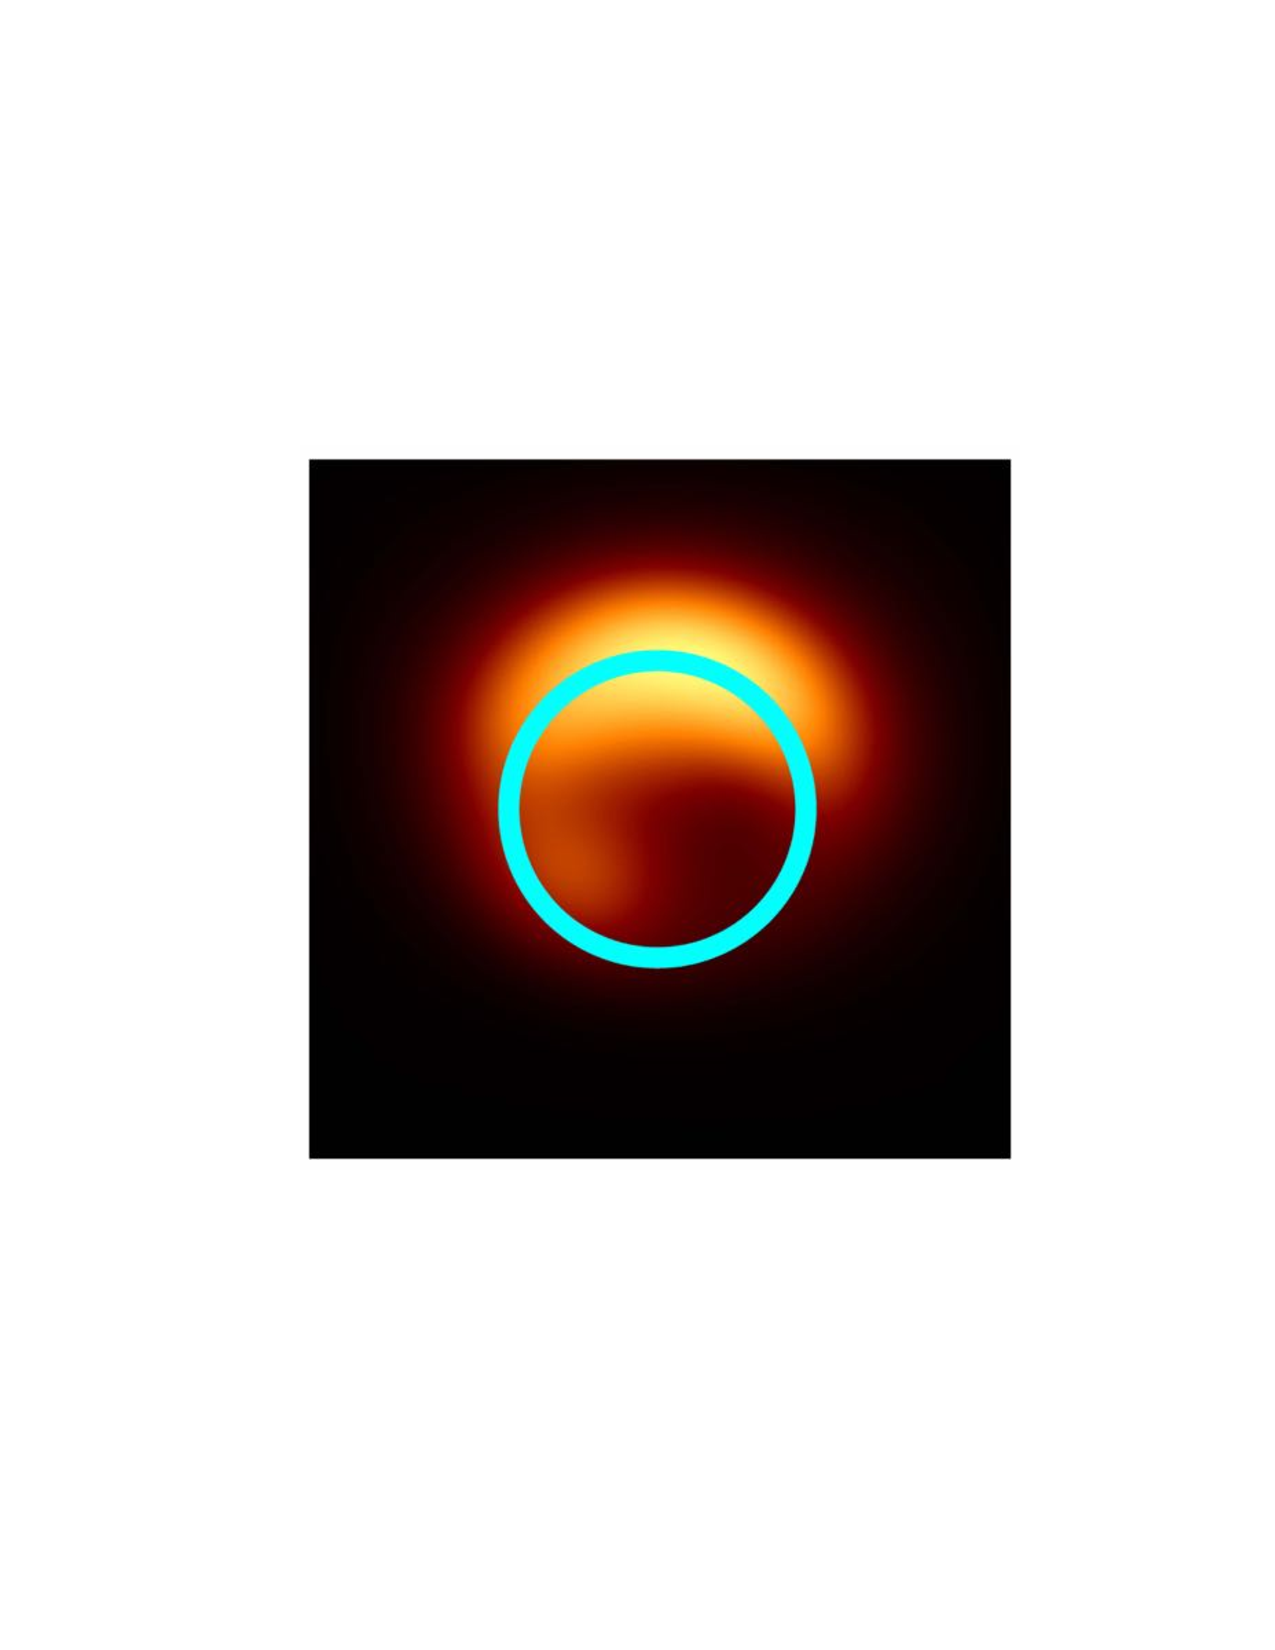
\includegraphics[height=.2\linewidth]{figures/hotspotcircleinterp/groundtruth_blur.pdf}} } &
			
\includegraphics[height=.2\linewidth]{figures/hotspotcircleinterp/groundtruth_blur.png} 
			\\
			&\vspace{-.1in}&\\
			\multirow{1}{*}[0.6in]{ \rotatebox[origin=t]{90}{\small{\textsf{ Snapshot }} }}
			&
			{{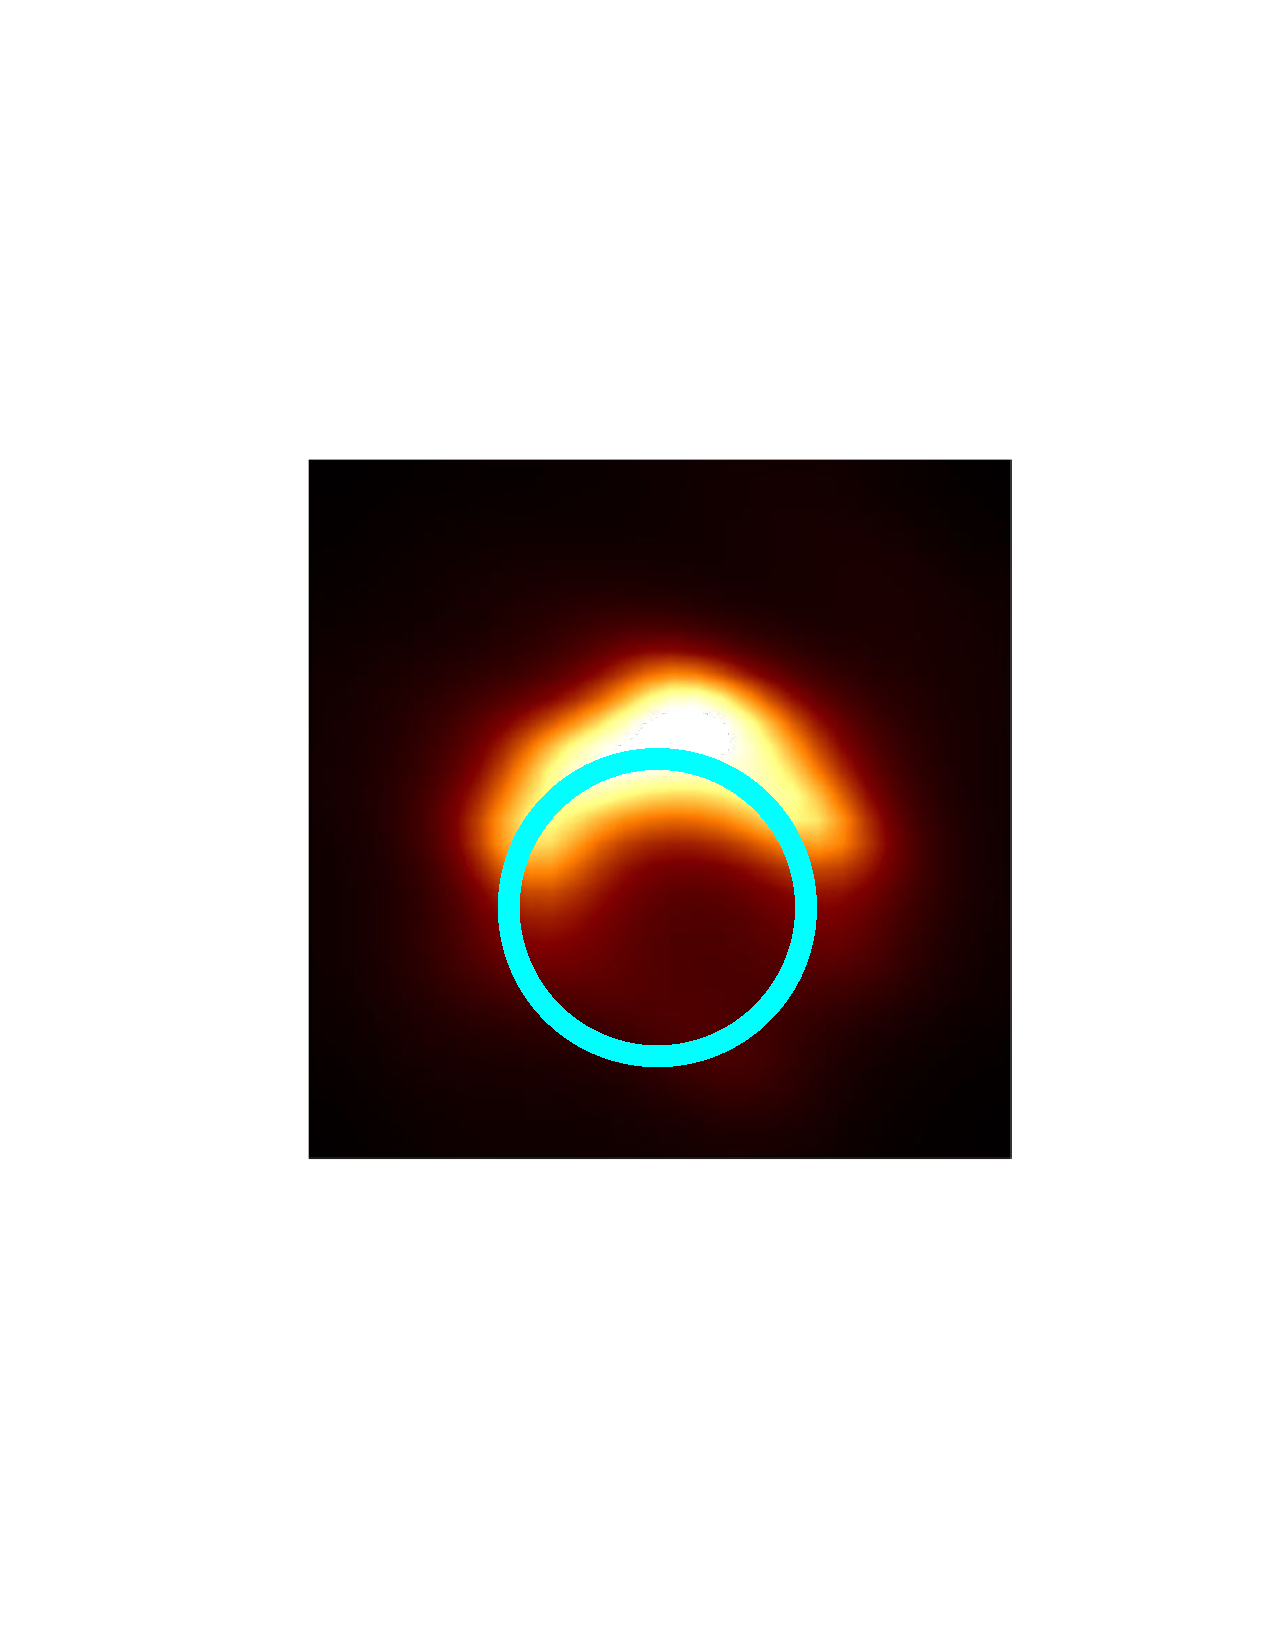
\includegraphics[height=.2\linewidth]{figures/hotspotcircleinterp/snapshot.pdf}} } &
			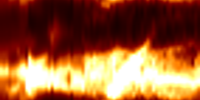
\includegraphics[height=.2\linewidth]{figures/hotspotcircleinterp/snapshot.png} 
			\\
				&\vspace{-.1in}&\\
					\multirow{1}{*}[0.65in]{ \rotatebox[origin=t]{90}{  \specialcell{ \small{\textsf{StarWarps:}} \\  \small{\textsf{No Warp}}}  }}
				&
				{{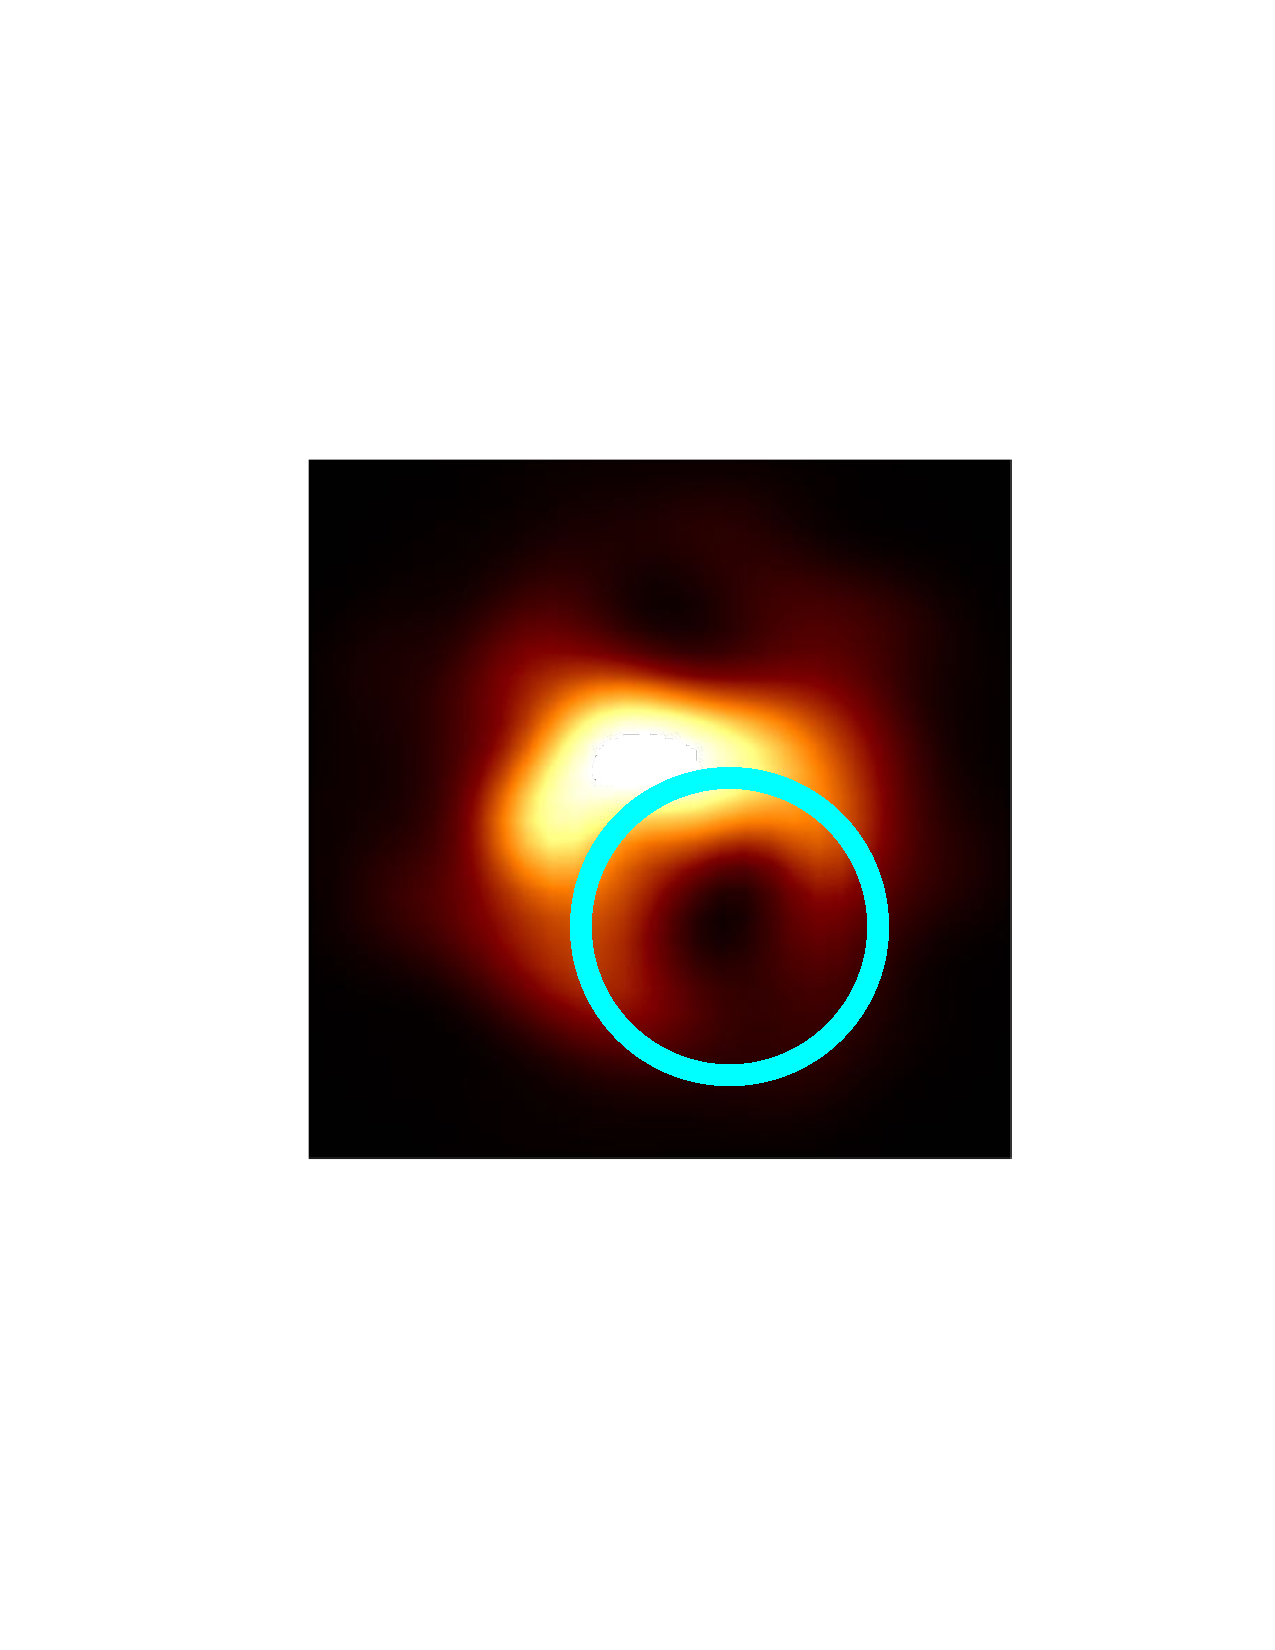
\includegraphics[height=.2\linewidth]{figures/hotspotcircleinterp/nomotion.pdf}} } &
				
\includegraphics[height=.2\linewidth]{figures/hotspotcircleinterp/nomotion.png} 
				\\
				&\vspace{-.1in}&\\
				\multirow{1}{*}[0.65in]{ \rotatebox[origin=t]{90}{  \specialcell{ \small{\textsf{StarWarps:}} \\  \small{\textsf{Learn Warp}}}  }}
				&
				{{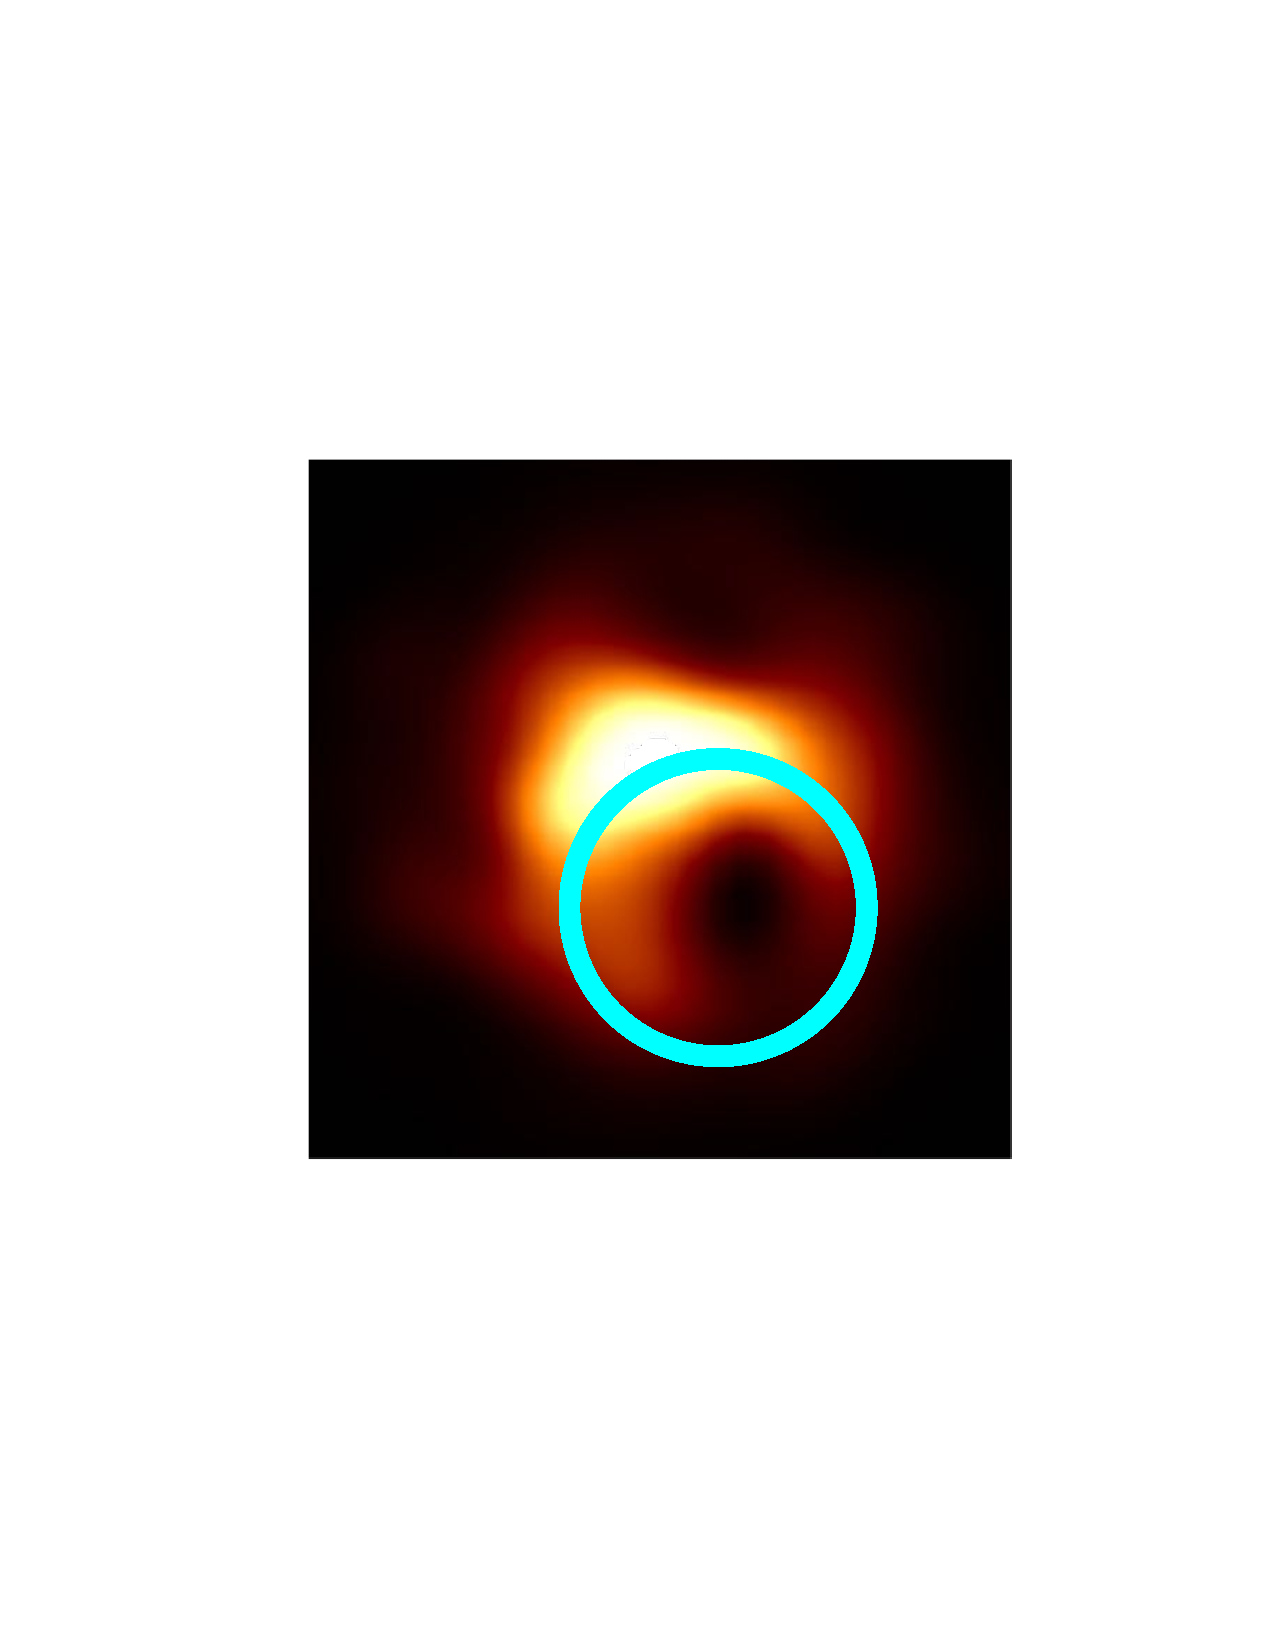
\includegraphics[height=.2\linewidth]{figures/hotspotcircleinterp/best.pdf}} } &
				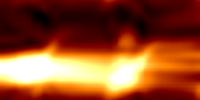
\includegraphics[height=.2\linewidth]{figures/hotspotcircleinterp/best.png} 
				\\
		\end{tabular}
		\caption{{\bf Visualizing Recovered Motion:} We visualize the recovered motion in Video 2 by displaying the change in intensity around a circle in the image over time. After fitting a circle of constant radius to each video,  the intensities around the circle in each image are unwrapped and placed in a single column in the unwrapped space $\times$ time image. As the hot spot rotates around the black hole a distinctive line appears in the true angle $\times$ time image. These lines also appear in the StarWarps angle $\times$ time images, but are harder to discern among the other artifacts in the snapshot imaging result. Results were obtained using the EHT2017+ array with added atmospheric noise, and correspond to results shown in Figure 2 of the supplemental document. As the absolute position of the source is lost when using the closure phase or bispectrum, the position of the recovered black hole moves slightly over the course of the video. This causes the fluctuation in the intensity of the bright horizontal line in the StarWarps recovered angle $\times$ time images, as we do not shift the position of the fitted circle.  }
		\label{fig:motion}
	\end{center}
	\vspace{-.35in}
\end{figure}
